% For SAPlugin diagrams
\usepackage{rotating}
\usepackage{pdflscape}
\usepackage{amsmath}
\usepackage{minitoc}
\usepackage[sort]{cleveref}
\usepackage{xparse}
\usepackage{expl3}
\usepackage{enumitem}
\usepackage{minitoc}
\usepackage{advdate}
\usepackage{pdftexcmds,xparse}
\usepackage{totcount}
\usepackage{lcg}
\usepackage{fontawesome}
\usepackage{tikz,pgfplots}
\usetikzlibrary{positioning,fit}
\usetikzlibrary{arrows}

% item labels
\makeatletter
\def\vpeitemlabel#1#2{\begingroup
	#2%
	\def\@currentlabel{#2}%
	\phantomsection\label{#1}\endgroup
}
\makeatother

\newcommand*\vpejustify{%
	\fontdimen2\font=0.4em%
	\fontdimen3\font=0.8em%
	\fontdimen4\font=0.1em%
	\fontdimen7\font=1.0em%
	\hyphenchar\font=`\-\relax%
}
\newcommand{\vpett}[1]{\vpejustify{\texttt{#1}}}
% vpe operation
\newcommand{\vpeoperation}[1]{#1}

% vpe data type
\newcommand{\vpedatatype}[2]{\vpeitemlabel{#1}{\textbf{\textsf{#2}}}}

% vpe exception
\newcommand{\vpeexception}[2]{\vpeitemlabel{#1}{\textsl{#2}}}

\newcommand{\iconcomponent}{%
	\begin{tikzpicture}[scale=0.3,thin,baseline=-0.05ex]
	\draw (0,0) rectangle (0.4, 0.6);
	\draw [fill=white] (-0.1,0.40) rectangle +(0.25, 0.1);
	\draw [fill=white] (-0.1,0.22) rectangle +(0.25, 0.1);	
	\end{tikzpicture}%
}
\newcommand{\iconprovided}{%
	\begin{tikzpicture}[scale=0.25,thin,baseline=-0.25ex]
	\draw (0.60,0.25) circle [radius=0.25];
	\draw (0, 0.25) -- (0.35, 0.25);
	\end{tikzpicture}%
}
\newcommand{\iconrequired}{%
	\begin{tikzpicture}[scale=0.25,thin,baseline=-0.25ex]
	\draw (0.60,0) arc (270:90:0.25);
	\draw (0, 0.25) -- (0.35, 0.25);
	\end{tikzpicture}%
}
\newcommand{\iconinher}{%
	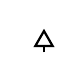
\begin{tikzpicture}[scale=0.3,thick,baseline=-0.5ex]
	\node (0,0) {};
	\draw[-open triangle 60] (.3,-.4) -- (.3, .6);
	\node (.9,0) {};
	\end{tikzpicture}%
}